\label{sec:overview}

A sketch of the testbed is depicted in Fig.~\ref{fig:testbed_setup}.
The testbed consists of up to 100 \ac{Raspi}s of different models.
More specifically, in our design we consider: Raspberry Pi 1 model B rev.~2,
Raspberry Pi 2 model B V1.1 and Raspberry Pi 3 model B V1.2.
All \ac{Raspi}s are each equipped with a 8 GB \ac{SD} memory card, a wired and wireless
network interface and a power supply. All the \ac{Raspi} are connected to
a common \ac{LAN} that provides internal and external connectivity. Without
loss of generality, in our case they are connected to a university network
using their wired Ethernet interface that is named \texttt{eth0} according
to the legacy naming convention of Ethernet interfaces in
Linux~\cite{PredictableNetworkInterfaceNames}. We consider the
university network since our testbed is used by students and academic staff
to perform measurements and experimentation of controlled and
reproducible scenarios as part of academic research. The
testbed description and procedures for setting it up are not restricted
to this academic scenario. All \ac{Raspi}s are configured to run
a \ac{SSH} daemon for easy remote access within the university network.
We requested the university \ac{IT} department to configure the university
\ac{DHCP} server to assign each \ac{Raspi} a static \ac{IP} address. This
eliminates the demand for monitors and keyboards with the \ac{Raspi}s
for non-graphical applications. Finally, our design aims to configure all
\ac{Raspi}s identically from a customized bootable image in their
respective memory cards, while still allowing the end-users to store
files locally in each of the \ac{Raspi}s.

\begin{figure}[ht!]
\centering
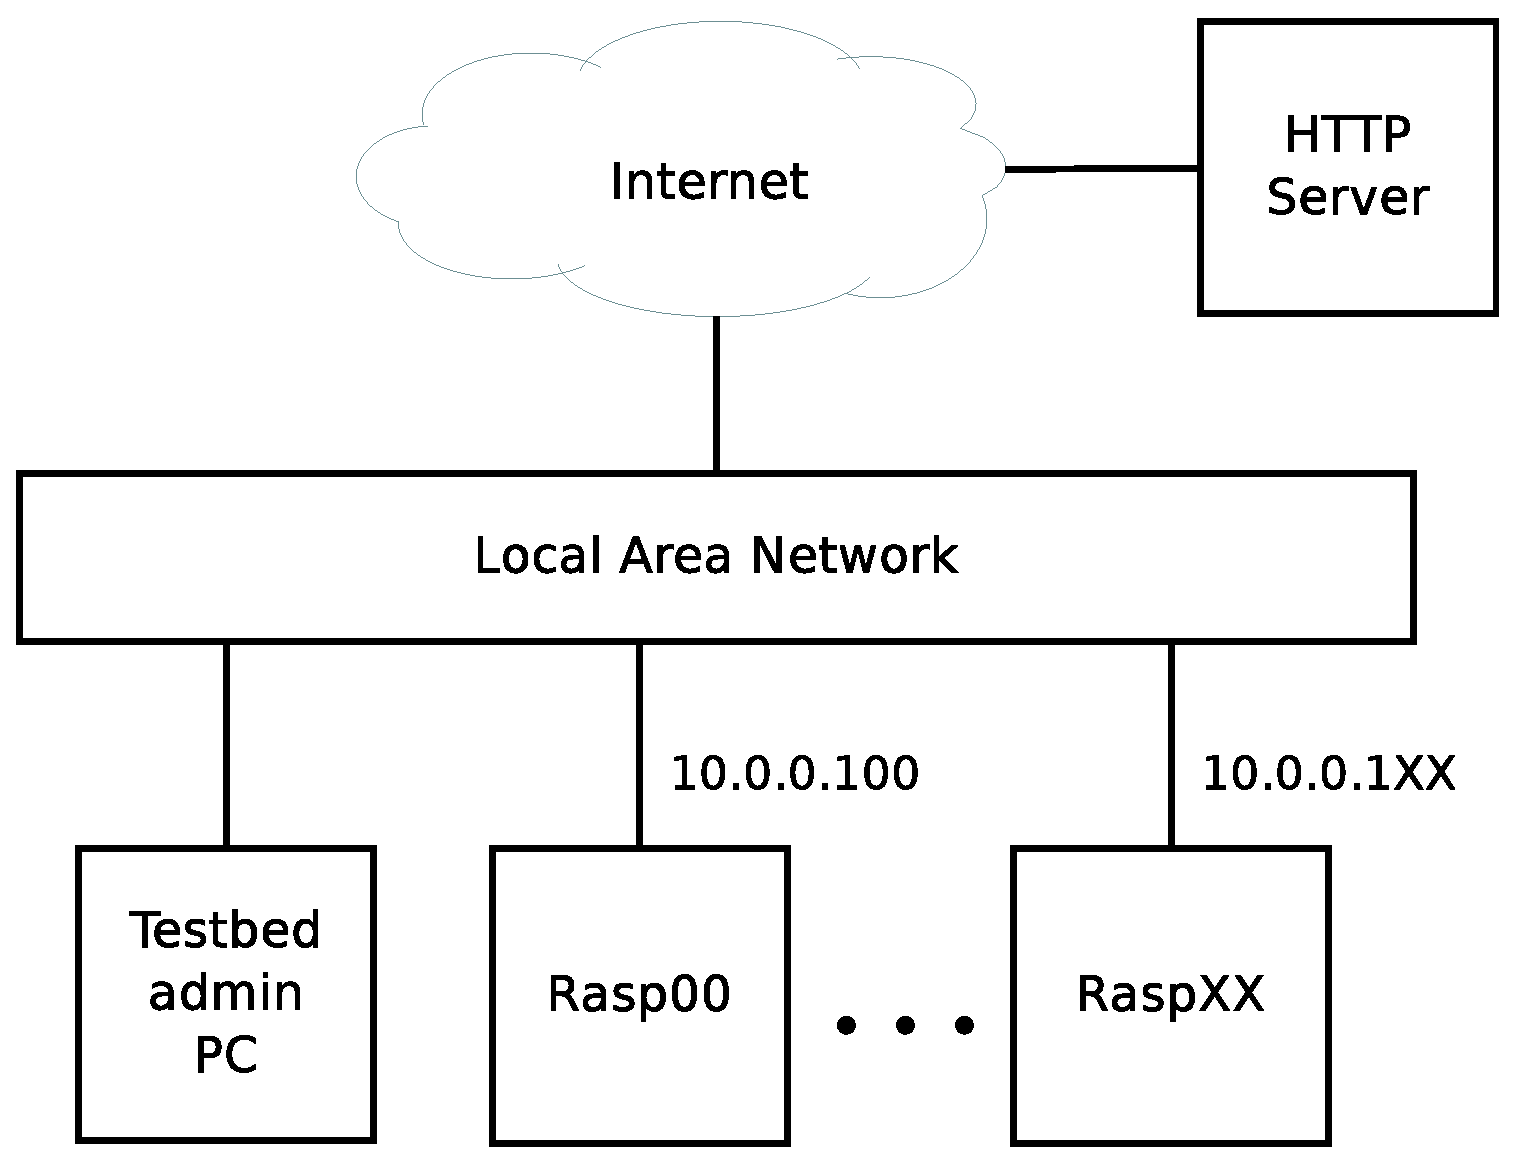
\includegraphics[width=0.42\textwidth]{images/testbed_setup3.eps}
\caption{Testbed setup}
\label{fig:testbed_setup}
\end{figure}

%This significantly eases the management of the \ac{Raspi}s
%as \ac{SSH} eliminates the need for monitors and keyboards for the \ac{Raspi}s.

We will refer to the
testbed administrator as the person(s) in charge of setting up and
configuring the testbed with administrator privileges from the \ac{OS}
point of view. The setting and configuration procedures are
performed by the testbed administrator in a \ac{PC} running a
Linux distribution as shown in Fig.~\ref{fig:testbed_setup}. Although in principle the administrator
Linux distribution is not a restriction, we present our procedure in a
Debian-based Linux distribution. Our basic design considers to create
a customized image to store it later on a memory card for each \ac{Raspi}.
Once configured, we store the resulting image file in a \ac{HTTP} server
as backup and in case the testbed administrator requires to make new
changes to this file.
%In our case, we use the university \ac{HTTP} server but any others can be used.
In our case, we store all files at Zenodo~\cite{soerensen_chres_wiant_2016_154143}, but the testbed administrator should copy the our files to his / her own \ac{HTTP} server to get read/write permissions.
We also put all the required
configuration files and scripts for the \ac{Raspi}s setup in the \ac{HTTP}
server so there is a single place where system setup is stored and could be
modified. This simplifies the system maintenance, as it may not always be desirable to make persistent changes
on the \ac{Raspi}s. For example when different users are interested in
running experiments on a rebooted testbed. We later present how
to utilize stacked filesystems to enable both persistent and
temporary storage to have this capability. Its purpose is to
remove non-desired data after a reboot while keeping the original
customized image structure. This step of the procedure is optional if
the testbed administrator decides to keep only persistent changes regardless
of the testbed use. Finally, we include a set of automation, monitoring
and cross-compilation tools over the top of our system in order to simplify
the execution of repetitive and long tasks, be able to follow the progress
of long task processes and compile relevant C++ source code for the testbed
administrator.


%an advanced step in our design considers to
% fetch the \ac{Raspi}s root filesystem from a \ac{HTTP} server. This enables the
% testbed administrator to put the data files in one location. The
% \ac{Raspi}s will then get these data files after a reboot. We consider
% that this step is particularly useful when there is a large amount
% of devices to be configured and the setup process needs to be automated.
% However, since a more complex scenario that might be required only in special
% cases, we put this step in Section~\ref{sec:http} in the Appendix.
